% !TEX root = ../rapport.tex

\newpage
\section{Idégenerering}
For at opnå den hurtigste omgangstid skal der være en kombination af den rigtige fysiske opsætning af bilen og en mikrocontroller der fortæller bilen hvordan den skal køre på banen.
Det første der blev undersøgt var de fysiske optimeringer der kunne laves på bilen.
\begin{itemize}
\item Forøgelse af acceleration og tophastighed
\item Formindskelse af bremselængde
\item Optimering hastighed igennem sving
\end{itemize}
For at optimere ovenstående er der flere ting der kan overvejes, se figur \ref{fig:mindmap1}.

\begin{figure}[ht]
    \centering
    \includegraphics[width=1\textwidth]{kapitler/billeder/Mindmap1.jpg}
    \caption{Idégenerering til optimering af omgangstid}
    \label{fig:mindmap1}
\end{figure}

Udover de fysiske komponenter i bilen skal bilens omgangstid også optimeres ved hjælp af software.


\newpage

\begin{figure}[ht]
    \centering
    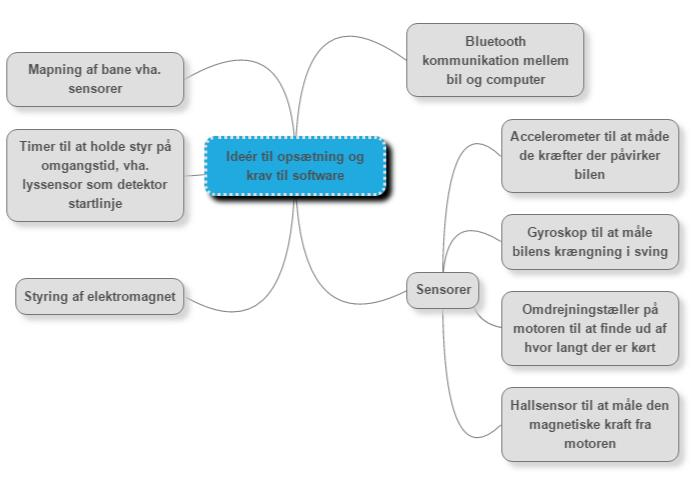
\includegraphics[width=0.8\textwidth]{kapitler/billeder/Mindmap2.jpg}
    \caption{Idégenerering til opsætning af software}
    \label{fig:mindmap2}
\end{figure}


Idéen er, at software skal kunne kortlægge den ukendte bane ved hjælp af sensorer, ved først at kører et par omgange.
Når banen er blevet kortlagt og gemt i bilens hukommelse kan den sætte en hurtig omgangs tid.
Mikrocontrolleren ved herefter, hvor og hvornår der er et sving, hvor der skal bremse og hvor hårdt den kan accelerere de forskellige steder på banen.
Idéen er altså, at bilen skal optimeres til at køre en så hurtig omgangstid som muligt, ved både at optimere det fysiske på bilen, dens hardware og software.
